% Author: Simon-Pierre Boucher — contact@spboucher.ai
%
% ═══════════════════════════════════════════════════════════════════════
% 3. DATA
% ═══════════════════════════════════════════════════════════════════════
\section{Data and Variable Construction}
\label{sec:data}

\subsection{Data Source}

The dataset is sourced from Zillow, the largest online real estate marketplace in the United States. The raw data contain 839,313 residential properties with 116 variables, representing active for-sale listings as of 2025--2026. The data include listing prices, structural characteristics, geocoordinates, neighborhood quality scores, and tax/transaction histories.

\textbf{Important limitations of the data source.} The sample comprises active Zillow listings, not the universe of U.S.\ residential properties. Several sources of non-representativeness should be noted: (i) Zillow coverage varies by region, with some MLS-linked markets better represented than others; (ii) active listings capture supply at a point in time, not the full housing stock; (iii) the sample excludes off-market properties, FSBOs not listed on Zillow, and recently transacted properties that are no longer listed; (iv) Southern states are overrepresented (56.6\% of the sample vs.\ approximately 38\% of U.S.\ housing units), likely reflecting higher listing volumes in fast-growing Sun Belt markets. We do not claim national representativeness and caution against interpreting our estimates as population parameters for the entire U.S.\ housing market.

\subsection{Listing Prices versus Transaction Prices}

A critical limitation is that our dependent variable is the \textit{listing} (asking) price, not the realized transaction price. Listing prices reflect seller expectations and strategic pricing behavior, not necessarily market-clearing values. List-to-sale price ratios vary by market condition, property type, and price tier: luxury properties are more frequently overpriced, distressed properties may be strategically underpriced, and regional norms for overbidding versus negotiation differ substantially \citep{knight2002listing}. Throughout this paper, we interpret the estimated coefficients as \textbf{listing-price capitalization gradients}---conditional associations between attributes and asking prices---rather than transaction-price implicit prices. If listing premiums correlate systematically with property attributes (e.g., if waterfront properties are more frequently overpriced), the estimated gradients will reflect this pricing behavior in addition to underlying valuation differences.

\subsection{Sample Construction}

Table~\ref{tab:attrition} documents the sample construction.

\begin{table}[H]
\centering
\caption{Sample Construction}
\label{tab:attrition}
\begin{threeparttable}
\begin{tabular}{lrrr}
\toprule
Step & $N$ remaining & Removed & Criterion \\
\midrule
Raw Zillow records & 839,313 & --- & --- \\
Valid price & 817,473 & 21,840 & $\$10{,}000 < P < \$10{,}000{,}000$ \\
Valid living area & 797,380 & 20,093 & $200 < \text{sqft} < 20{,}000$ \\
Valid bedrooms/bathrooms & 790,799 & 6,581 & $1 \leq \text{bed} \leq 10$, $1 \leq \text{bath} \leq 10$ \\
Valid geocoordinates & 789,199 & 1,600 & Non-missing lat/lon \\
U.S.\ states + DC only & 788,842 & 357 & Exclude PR, VI \\
\midrule
\textbf{Final analytical sample} & \textbf{788,842} & \textbf{50,471} & \textbf{(6.0\% removed)} \\
\bottomrule
\end{tabular}
\begin{tablenotes}
\small
\item \textit{Notes:} Filters applied sequentially. The 6.0\% removal rate suggests the raw data are reasonably clean, though the retained sample may still contain measurement error in secondary variables.
\end{tablenotes}
\end{threeparttable}
\end{table}

\subsection{Variable Description}

Our specification includes 62 regressors organized into six categories.

\subsubsection{Structural Attributes (8 Variables)}

The natural logarithm of living area ($\ln\text{sqft}$), number of bedrooms, number of bathrooms, property age ($2026 - \text{year\_built}$) and its square, number of stories, the bathroom-to-bedroom ratio, and square feet per bedroom. Living area enters in log form to accommodate the well-documented concavity of the size-price relationship.

\subsubsection{Lot Characteristics (1 Variable)}

The natural logarithm of lot size ($\ln\text{lot}$). Missing lot sizes (16.3\% of raw data) are imputed using state-level medians.

\subsubsection{Amenity and Quality Indicators (11 Variables)}

Binary indicators for swimming pool (39.8\% prevalence), spa (6.1\%), basement (24.3\%), fireplace (39.6\%), garage (67.2\%), waterfront location (8.9\%), central air conditioning (68.1\%), forced air heating (25.8\%), and hardwood flooring (26.7\%). The number of parking spaces and a composite luxury score (0--7) supplement these indicators.

\subsubsection{Neighborhood and Location Variables (7 Variables)}

Walk Score (0--100), Bike Score, Transit Score, average GreatSchools rating (1--10), school count, distance to nearest school, and local property tax rate.

\textbf{Data quality note.} Bike Score has a maximum value of 248 in our data, exceeding the expected 0--100 range. Only 38 observations (0.005\%) exceed 100, and these are retained without truncation. Results are robust to capping Bike Score at 100.

\subsubsection{Market Status Variables (5 Variables)}

Condominium indicator (14.6\%), HOA membership (37.1\%), log annualized HOA fees ($\ln(1 + \text{HOA}_\text{annual})$), new construction (5.9\%), and foreclosure status (0.5\%).

\subsubsection{Interaction Terms (6 Variables)}

\begin{itemize}[nosep]
    \item $\ln(\text{sqft}) \times \text{age}$: depreciation-size interaction;
    \item $\text{pool} \times \text{South}$: climate-dependent pool gradient;
    \item $\text{waterfront} \times \ln(\text{sqft})$: size-dependent waterfront gradient;
    \item $\text{basement} \times \text{North}$: region-dependent basement gradient;
    \item $\text{condo} \times \text{walk\_score}$: walkability gradient for condominiums;
    \item $\text{age} \times \text{luxury\_score}$: luxury mitigation of depreciation.
\end{itemize}

\subsubsection{Categorical Controls (24 Dummy Variables)}

Simplified indicators for roof type (6 dummies), construction material (8 dummies), foundation type (7 dummies), and Census region (3 dummies; Midwest reference).

\subsection{Missing Data and Imputation}

Table~\ref{tab:missing} reports missingness rates for key variables.

\begin{table}[H]
\centering
\caption{Missing Data Rates and Imputation Methods}
\label{tab:missing}
\begin{threeparttable}
\small
\begin{tabular}{lrrl}
\toprule
Variable & Missing (\%) & Method & Notes \\
\midrule
Year built & 19.4 & State median & Affects age, age$^2$, interactions \\
Lot size & 16.3 & State median & Large variation \\
Walk Score & 3.1 & State median & \\
Bike Score & 6.1 & State median & Max = 248 (38 obs.) \\
Transit Score & 70.1 & Set to 0 & Suburban/rural properties \\
Garage & 35.1 & Set to False & Conservative \\
Climate risk factors & 100.0 & Excluded & Not available \\
\bottomrule
\end{tabular}
\begin{tablenotes}
\small
\item \textit{Notes:} State-level median imputation is used to preserve geographic variation. The high Transit Score missingness (70.1\%) likely reflects properties in areas without public transit infrastructure, for which zero is a reasonable value. Climate risk factors (flood, fire, heat, wind, air) are entirely missing and excluded from the analysis.
\end{tablenotes}
\end{threeparttable}
\end{table}

\subsection{Data Quality Audit}
\label{sec:data_audit}

We conduct three data quality checks to assess the sensitivity of key results to imputation and outliers.

\textbf{Imputation prevalence.} Two variables---year built (19.4\% missing) and lot size (16.3\% missing)---account for the bulk of imputed values. To assess the consequences, we re-estimate the baseline OLS model on subsamples that exclude imputed observations (Section~\ref{sec:imputation_sensitivity}). The lot-size coefficient is the most sensitive: $\ln(\text{lot})$ triples from 0.018 to 0.059 when imputed lot sizes are dropped, suggesting that state-median imputation attenuates the lot-size gradient substantially.

\textbf{Outlier prevalence.} We winsorize lot size at its 99.5th percentile and cap Bike Score at 100, then re-estimate OLS (Section~\ref{sec:winsorization}). The overall $R^2$ increases modestly from 0.634 to 0.640, and most coefficients are stable, with the exception of $\ln(\text{lot})$, which again increases substantially.

\textbf{Geographic coverage.} The sample spans 886 unique three-digit ZIP code prefixes (ZIP3 codes) across 51 jurisdictions (50 states plus DC). Southern states account for 56.6\% of observations. We document the marginal explanatory power of progressively finer geographic controls in Section~\ref{sec:ols_fe}.

\subsection{Descriptive Statistics}

Table~\ref{tab:descriptive} presents summary statistics.

\begin{table}[H]
\centering
\caption{Descriptive Statistics ($N = 788{,}842$)}
\label{tab:descriptive}
\begin{threeparttable}
\small
\begin{tabular}{lrrrrrr}
\toprule
Variable & Mean & Std.\ Dev. & Min & Median & Max \\
\midrule
\multicolumn{6}{l}{\textit{Continuous Variables}} \\
Listing Price (\$) & 621,737 & 817,965 & 10,300 & 399,900 & 9,999,999 \\
Living Area (sqft) & 2,093 & 1,181 & 208 & 1,820 & 19,600 \\
Bedrooms & 3.25 & 1.09 & 1 & 3 & 10 \\
Bathrooms & 2.52 & 1.16 & 1 & 2 & 10 \\
Property Age (years) & 42.2 & 31.5 & 0 & 36 & 200 \\
Walk Score (0--100) & 25.6 & 26.5 & 0 & 16 & 100 \\
Bike Score & 34.9 & 18.1 & 1 & 31 & 248 \\
Transit Score (0--100) & 8.9 & 18.3 & 0 & 0 & 100 \\
Avg.\ School Rating (1--10) & 6.02 & 0.90 & 1 & 6 & 10 \\
Property Tax Rate (\%) & 1.10 & 0.53 & 0 & 1.0 & 4.0 \\
Luxury Score (0--7) & 1.36 & 1.29 & 0 & 1 & 7 \\
\midrule
\multicolumn{6}{l}{\textit{Binary Variables (prevalence)}} \\
Swimming Pool & 39.8\% & & & & \\
Garage & 67.2\% & & & & \\
Fireplace & 39.6\% & & & & \\
Basement & 24.3\% & & & & \\
Waterfront & 8.9\% & & & & \\
HOA & 37.1\% & & & & \\
Central Air & 68.1\% & & & & \\
Hardwood Floors & 26.7\% & & & & \\
Condominium & 14.6\% & & & & \\
New Construction & 5.9\% & & & & \\
Foreclosure & 0.5\% & & & & \\
\midrule
\multicolumn{6}{l}{\textit{Regional Distribution}} \\
South & 56.6\% & & & & \\
West & 18.9\% & & & & \\
Midwest & 16.1\% & & & & \\
Northeast & 8.4\% & & & & \\
\bottomrule
\end{tabular}
\begin{tablenotes}
\small
\item \textit{Notes:} Listing prices, not transaction prices. Property age computed as $2026 - \text{year\_built}$, after imputation. Imputed values included in summary statistics.
\end{tablenotes}
\end{threeparttable}
\end{table}

The median listing price is \$399,900, with substantial right-skewness (mean \$621,737). The log transformation substantially improves distributional symmetry (Figure~\ref{fig:price_dist}), supporting the semi-log specification.

\begin{figure}[H]
    \centering
    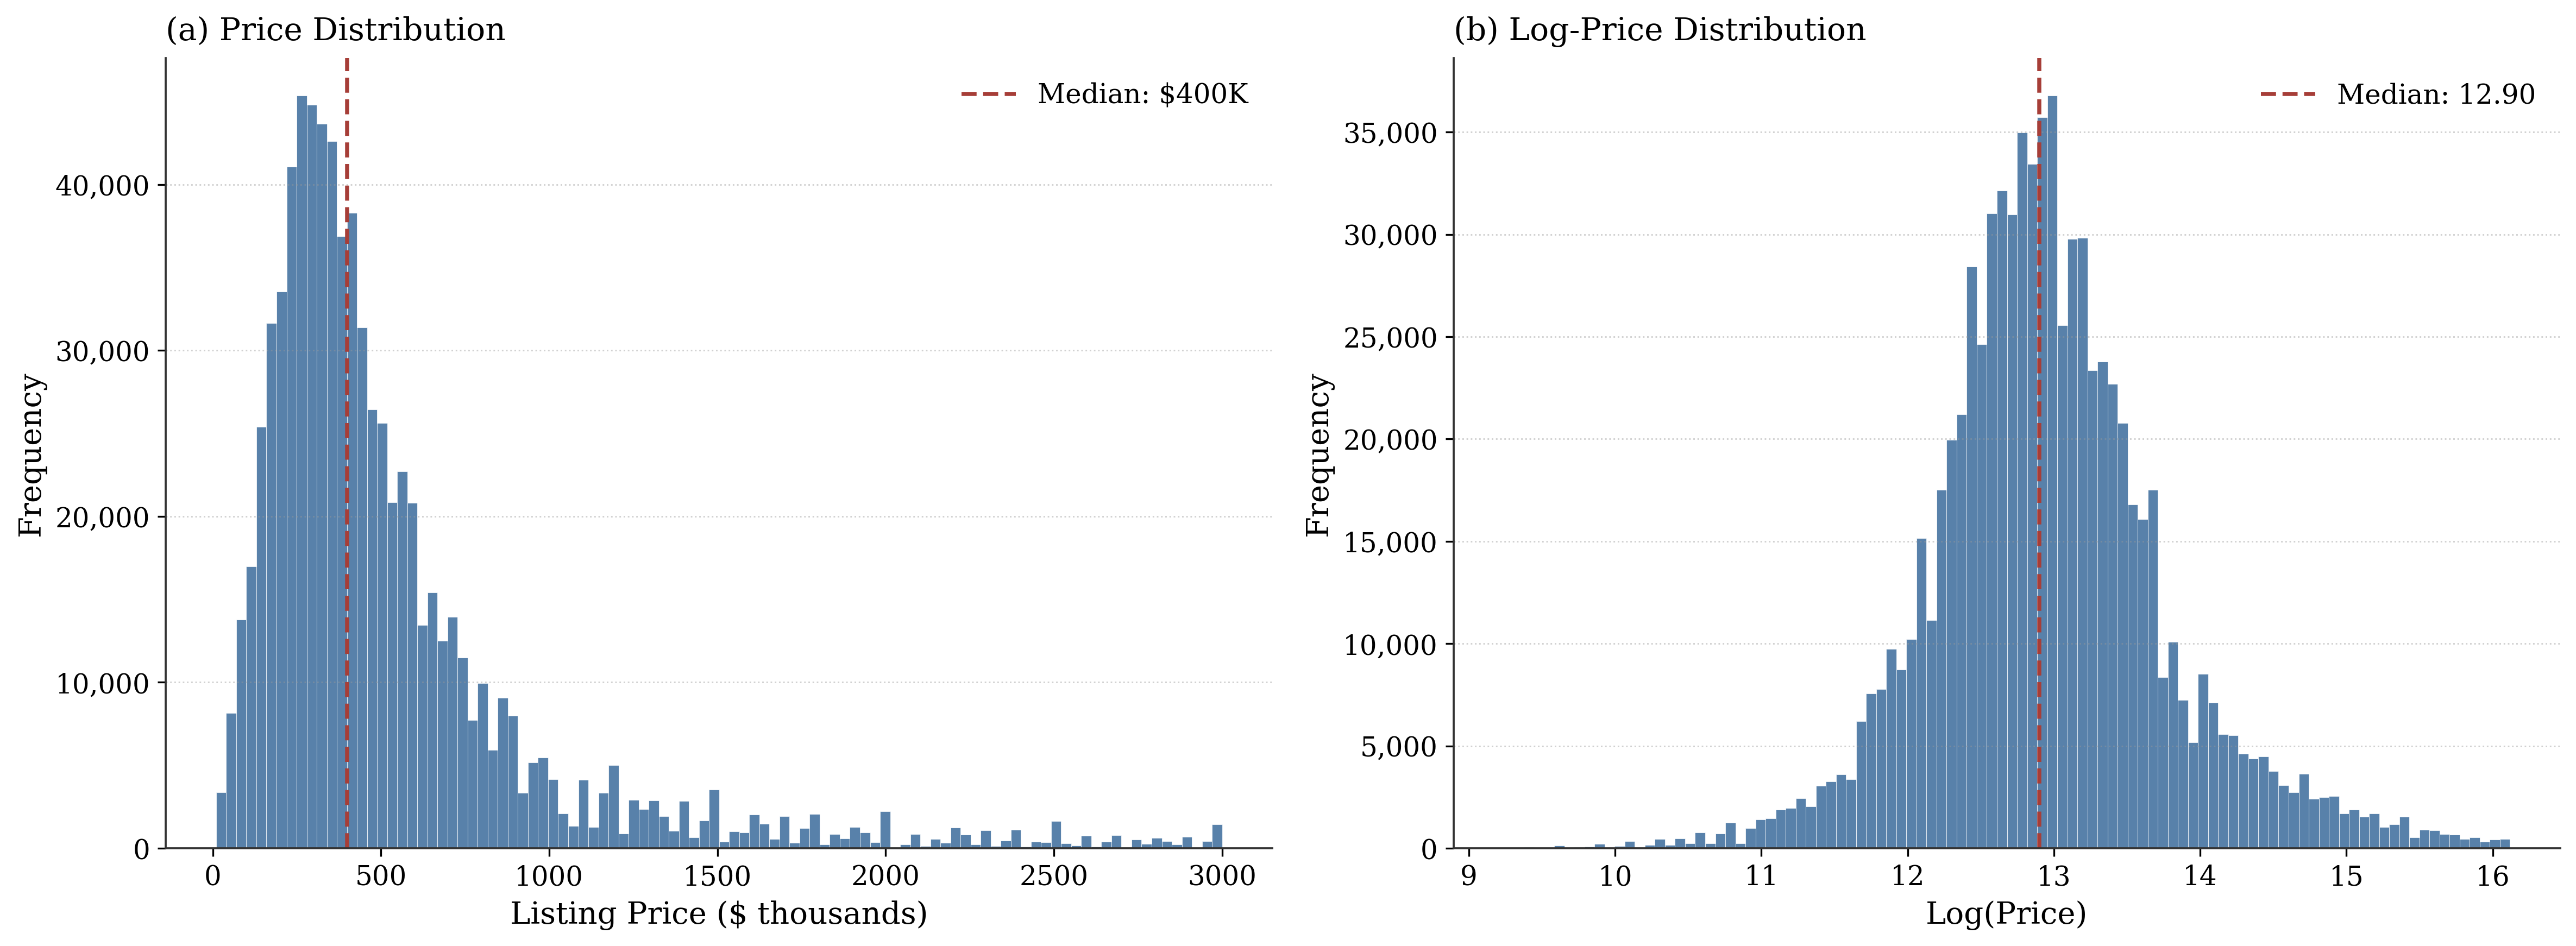
\includegraphics[width=\textwidth]{figures/fig1_price_distribution.png}
    \caption{Distribution of Listing Prices: (a) Levels; (b) Natural Logarithm. The log transformation reduces right skewness and approximates normality.}
    \label{fig:price_dist}
\end{figure}
